\appendix

\section{Appendix}

\subsection{Additional Figures}

\begin{figure}[!htpb]
   \centering
   \small
   \caption{}
   \label{fig:number_of_contracts_by_inst}
   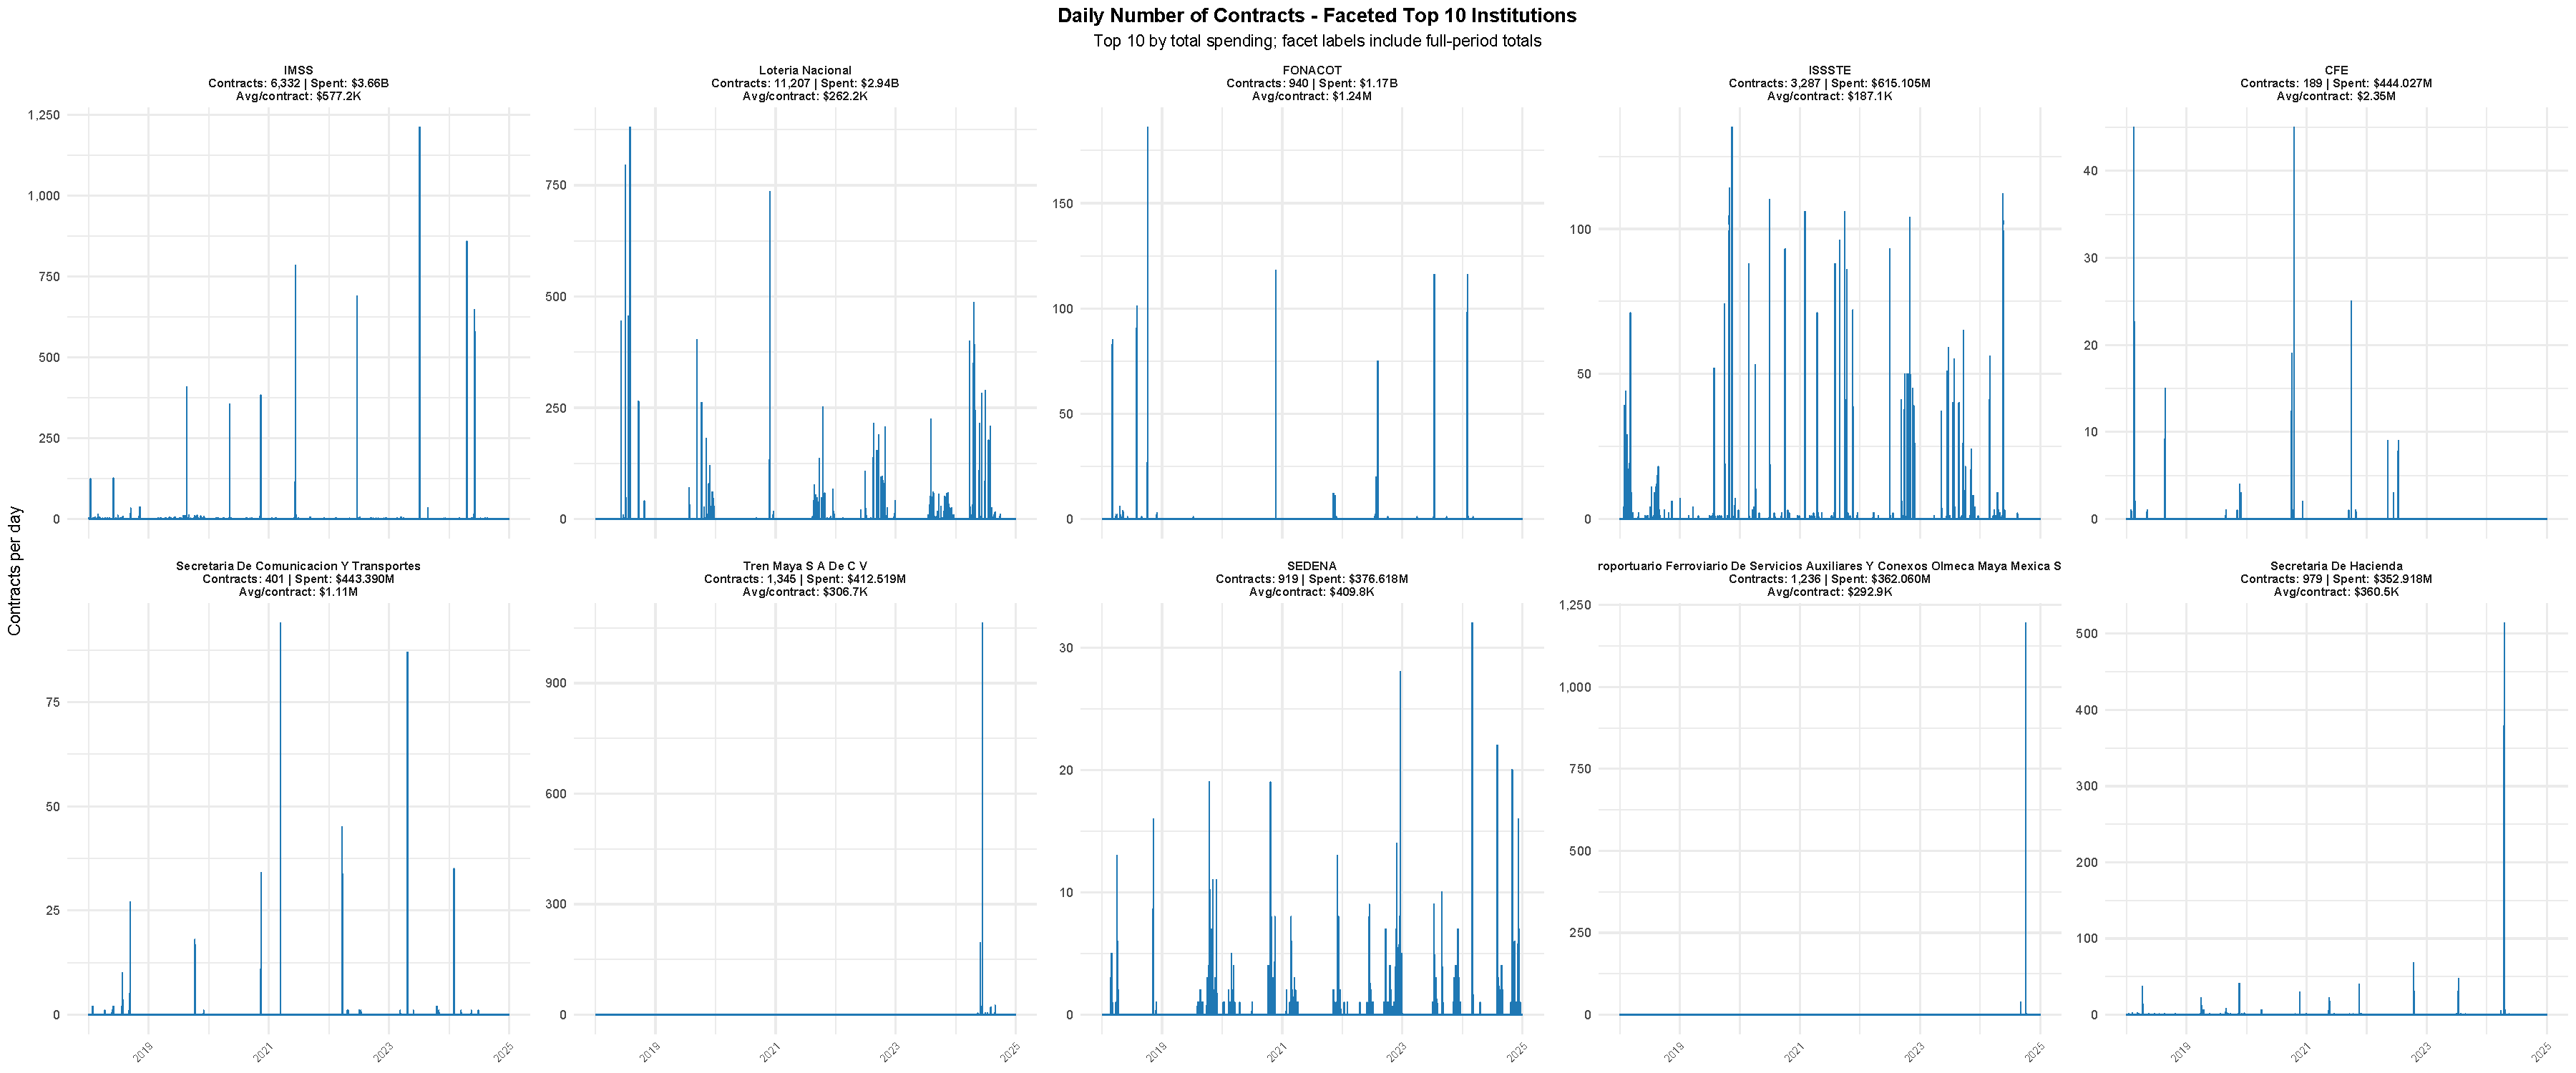
\includegraphics[width=1.1\textwidth]{figures/descriptive_stats/top10_institutions_daily_contracts_faceted.pdf}
   \caption*{ \footnotesize{\textit{Note:} This figure presents the number of contracts assigned to the top 10 institutions which assigned more contracts from 2018 to 2024 for the federal advertising spending from the Mexican government. Data was obtained from COMSOC}}
\end{figure}

\subsection{Proofs}

\subsection{Utility derivation}
\label{sec:utility}

The government chooses advertising discipline $\phi \geq 0$ before the conference. 
A higher value of $\phi$ increases the probability that media outlets ask friendly 
questions, but it is also costly for the government. The government values public 
engagement, denoted by $V>0$, and pays a marginal cost of discipline $\kappa>0$.

The probability that the public observes the scripted signal $S$ is
\begin{equation}
    \Pr(S)
    =
    \Pr(S \mid G)\Pr(G) + \Pr(S \mid B)\Pr(B).
\end{equation}

Under the assumptions of the model, $\Pr(S \mid G)=1$, $\Pr(G)=q$, 
$\Pr(B)=1-q$, and $\Pr(S \mid B)=\beta_t(\phi)$. Therefore,
\begin{equation}
    \Pr(S)
    =
    1\cdot q + \beta_t(\phi)(1-q),
\end{equation}
which implies
\begin{equation}
    \Pr(S)
    =
    q + (1-q)\beta_t(\phi).
\end{equation}

Thus, the government's expected benefit from public engagement is
\begin{equation}
    \left[q+(1-q)\beta_t(\phi)\right]V.
\end{equation}

However, this benefit is obtained only if the scripted signal remains credible. 
That is, the public engages only when
\begin{equation}
    \beta_t(\phi) \leq \beta^*,
\end{equation}
where $\beta^*$ is the maximum level of scripted-looking behavior that remains 
consistent with public engagement. Hence, the government's problem is
\begin{equation}
    \max_{\phi \geq 0} \;
    \left[q+(1-q)\beta_t(\phi)\right]V
    \cdot \ind\{\beta_t(\phi)\leq \beta^*\}
    -\kappa\phi.
\end{equation}

In the benchmark case,
\begin{equation}
    \beta_t(\phi)=\Phi(\gamma\phi-\Delta_N).
\end{equation}

Substituting this expression into the government's objective gives
\begin{equation}
    \max_{\phi \geq 0} \;
    \left[q+(1-q)\Phi(\gamma\phi-\Delta_N)\right]V
    \cdot \ind\{\Phi(\gamma\phi-\Delta_N)\leq \beta^*\}
    -\kappa\phi.
\end{equation}

The credibility constraint requires
\begin{equation}
    \Phi(\gamma\phi-\Delta_N)\leq \beta^*.
\end{equation}

Since $\Phi(\cdot)$ is strictly increasing, applying the inverse normal CDF gives
\begin{equation}
    \gamma\phi-\Delta_N \leq \Phi^{-1}(\beta^*).
\end{equation}

Solving for $\phi$ yields
\begin{equation}
    \phi \leq \frac{\Delta_N+\Phi^{-1}(\beta^*)}{\gamma}.
\end{equation}

Define this upper bound as
\begin{equation}
    \phi_{\max}
    =
    \frac{\Delta_N+\Phi^{-1}(\beta^*)}{\gamma}.
\end{equation}

Therefore, instead of writing the credibility condition as an indicator function, 
we can restrict the government's choice set to the feasible interval 
$\phi \in [0,\phi_{\max}]$. The benchmark government problem becomes
\begin{equation}
    \max_{\phi \in [0,\phi_{\max}]} \;
    V_G(\phi)
    =
    \left[q+(1-q)\Phi(\gamma\phi-\Delta_N)\right]V
    -\kappa\phi.
\end{equation}

\subsection{Proof of Proposition 1}

The public engages after observing $S$ if and only if
\begin{equation}
    \Prob(G\mid S)\geq \tau.
\end{equation}
Using Bayes' rule and Assumption 1,
\begin{equation}
    \Prob(G\mid S)=\frac{\Prob(S\mid G)\Prob(G)}{\Prob(S)}
    =\frac{q}{q+(1-q)\beta_t}.
\end{equation}
Therefore, engagement after $S$ requires
\begin{equation}
    \frac{q}{q+(1-q)\beta_t}\geq \tau.
\end{equation}
Multiplying both sides by the positive denominator gives
\begin{equation}
    q \geq \tau[q+(1-q)\beta_t].
\end{equation}
Rearranging,
\begin{equation}
    q(1-\tau) \geq \tau(1-q)\beta_t.
\end{equation}
Since $\tau(1-q)>0$, this implies
\begin{equation}
    \beta_t \leq \frac{q(1-\tau)}{\tau(1-q)}\equiv \beta^*.
\end{equation}
Finally, since $q<\tau$, it follows that $\beta^*<1$. Thus, full suppression, $\beta_t=1$, violates the credibility constraint. \qed

\subsection{Proof of Proposition 2}

An outlet asks a critical question when the payoff from criticism exceeds the payoff from a friendly question:
\begin{equation}
    \Delta_{t_i}+\varepsilon_{it} > \gamma\phi.
\end{equation}
Equivalently,
\begin{equation}
    \varepsilon_{it}>\gamma\phi-\Delta_{t_i}.
\end{equation}
Since $\varepsilon_{it}\sim\mathcal{N}(0,1)$,
\begin{equation}
    p_{t_i}(\phi)=\Prob(\varepsilon_{it}>\gamma\phi-\Delta_{t_i})
    =\Phi(\Delta_{t_i}-\gamma\phi).
\end{equation}
Differentiating with respect to $\phi$ yields
\begin{equation}
    \frac{\partial p_{t_i}(\phi)}{\partial \phi}=-\gamma n(\Delta_{t_i}-\gamma\phi)<0.
\end{equation}
If $\Delta_N>\Delta_A$, then $\Phi(\Delta_N-\gamma\phi)>\Phi(\Delta_A-\gamma\phi)$ for any fixed $\phi$, so $p_N(\phi)>p_A(\phi)$. \qed

\subsection{Proof of Proposition 3}

In the benchmark case, one non-aligned outlet receives the microphone in the unfavorable state. The conference appears scripted in the bad state if and only if that outlet asks a friendly question. Therefore,
\begin{equation}
    \beta_t(\phi)=\Prob(c_{it}=0\mid Ask_{it}=1,t_i=N).
\end{equation}
Since $p_N(\phi)=\Prob(c_{it}=1\mid Ask_{it}=1,t_i=N)$,
\begin{equation}
    \beta_t(\phi)=1-p_N(\phi)=1-\Phi(\Delta_N-\gamma\phi).
\end{equation}
By symmetry of the standard normal distribution,
\begin{equation}
    1-\Phi(\Delta_N-\gamma\phi)=\Phi(\gamma\phi-\Delta_N).
\end{equation}
Thus,
\begin{equation}
    \beta_t(\phi)=\Phi(\gamma\phi-\Delta_N).
\end{equation}
Differentiating,
\begin{equation}
    \frac{\partial \beta_t(\phi)}{\partial \phi}=\gamma \Phi'(\gamma\phi-\Delta_N)>0.
\end{equation}
\qed

\subsection{Proof of Proposition 4}

The government's objective on the credibility-feasible region is
\begin{equation}
    V_G(\phi)=\left[q+(1-q)\Phi(\gamma\phi-\Delta_N)\right]V-\kappa\phi,
\end{equation}
with $\phi\in[0,\phi_{\max}]$. The first derivative is
\begin{equation}
    \frac{\partial V_G}{\partial \phi}=(1-q)\gamma V n(\gamma\phi-\Delta_N)-\kappa.
\end{equation}
Define
\begin{equation}
    k\equiv \frac{\kappa}{(1-q)\gamma V}, \qquad z\equiv \gamma\phi-\Delta_N.
\end{equation}
The first-order condition is
\begin{equation}
    n(z)=k.
\end{equation}
Since $n(z)=(1/\sqrt{2\pi})\exp(-z^2/2)$, this equation has real solutions if and only if $k\leq 1/\sqrt{2\pi}$. When real solutions exist,
\begin{equation}
    z=\pm\sqrt{-2\ln(k\sqrt{2\pi})}.
\end{equation}
The second derivative is
\begin{equation}
    \frac{\partial^2 V_G}{\partial \phi^2}=-(1-q)\gamma^2V z n(z).
\end{equation}
A local maximum requires $z>0$. Therefore, the interior candidate is
\begin{equation}
    z^*=\sqrt{-2\ln(k\sqrt{2\pi})}, \qquad \phi^*=\frac{\Delta_N+z^*}{\gamma}.
\end{equation}

If $k>1/\sqrt{2\pi}$, the marginal benefit of discipline is everywhere below the marginal cost, so the government sets $\phi^*=0$. If $k\leq 1/\sqrt{2\pi}$ and the interior candidate satisfies the credibility constraint, then the interior solution is optimal. This requires
\begin{equation}
    \Phi(z^*)\leq \beta^*,
\end{equation}
which is equivalent to
\begin{equation}
    z^*\leq \Phi^{-1}(\beta^*).
\end{equation}
Since $n(z)$ is decreasing for $z>0$, this is equivalent to
\begin{equation}
    k\geq n(\Phi^{-1}(\beta^*)).
\end{equation}
If instead $k<n(\Phi^{-1}(\beta^*))$, the unconstrained optimum violates the credibility constraint, and the government chooses the boundary $\phi_{\max}$ such that $\beta_t(\phi_{\max})=\beta^*$. This gives
\begin{equation}
    \phi_{\max}=\frac{\Delta_N+\Phi^{-1}(\beta^*)}{\gamma}.
\end{equation}
These three cases establish the proposition. \qed

\subsection{Proof of Proposition 5}

In the interior equilibrium,
\begin{equation}
    n(z^*)=k=\frac{\kappa}{(1-q)\gamma V}, \qquad \beta_t^*=\Phi(z^*).
\end{equation}
Differentiating $n(z^*)=k$ gives
\begin{equation}
    n'(z^*)\frac{dz^*}{dk}=1.
\end{equation}
Since $n'(z)=-zn(z)$,
\begin{equation}
    \frac{dz^*}{dk}=-\frac{1}{z^*n(z^*)}<0.
\end{equation}
Because $\beta_t^*=\Phi(z^*)$, the sign of each comparative static follows from the effect of each parameter on $k$. Since $k$ is increasing in $\kappa$ and $q$, $\beta_t^*$ is decreasing in $\kappa$ and $q$. Since $k$ is decreasing in $\gamma$ and $V$, $\beta_t^*$ is increasing in $\gamma$ and $V$. Finally, $\Delta_N$ does not enter $k$, so $\partial \beta_t^*/\partial \Delta_N=0$. \qed